\chapter{node2vec Theoretical Study}\label{chap:1}
In this chapter we provide detailed description on node2vec embedding method. First, we get through exact process of embedding generation, then we outline algorithm hyperparameters. Last, we give an overview of existing algorithm implementations.

As we stated above graph embedding suggests representing network vertices into a low-dimensional vector space~\cite{cao2015grarep}:
\[
   f: V \rightarrow \mathbb{R}^d,
\]
chosen so that preserving information about network topology structure\cite{fortunato2010community}. Here $d$ is the number of dimensions of our feature representation. The above requirement can be expressed in terms of maximizing the likelihood of network neighborhoods preserving:
\[ 
    \max_f \sum_{u \in V} \log P(N_S(u)|f(u)).
\]

The objective can be efficiently optimized using stochastic gradient descent (SGD)~\cite{recht2011hogwild}.
The idea behind an embedding is that the neighborhood (the context) of each node to much extend determines the properties of the node itself.

Here we used the notion of node's neighborhood~\cite{adamic2003friends}, that must be clearly specified before we may continue. More formally, we have to define a sampling strategies. 

\textit{For each node $u \in V$, its network neighborhood $N_S (u) \subset V$ is generated through a neighborhood sampling strategy $S$.}

The simplest such strategies are, for instance, Breadth-first Sampling (BFS) and Depth-first Sampling (DFS), but being deterministic they represent single node's neighborhood, failing to preserve a complex structure of a node's neighborhood. Instead, the $node2vec$ approach, that we will work with, solves this by using randomized procedure to sample many different neighborhoods for a single node.

\section{Random Walks}

For each node $u$, consider the following random walk of the fixed length $\ell$ with the following distribution~\cite{DBLP:journals/corr/abs-1011-4071}:
\begin{equation*}
P(c_i = x|c_{i-1} = v) =
 \begin{cases}
   \pi_{vx}/Z &\text{if $(v,x)\in E$}\\
   0 &\text{ otherwise}
 \end{cases}
\end{equation*}
Here $Z$ is the normalizing constant, $\pi_{vx}$ is transition probability between nodes $v$ and $x$, defined as: 
\[ 
  \alpha _{pq}(t, x) = \begin{cases}
   1/p &\text{ if $d_{tx} = 0$}\\
   1   &\text{ if $d_{tx} = 1$}\\
   1/q &\text{ if $d_{tx} = 2$}
   \end{cases}
\]
where $d_{tx}$ denotes the shortest path distance between nodes $t$ and $x$.


The two parameters have the following meaning:

\begin{enumerate}
    \item return parameter $p$ --- controls the likelihood of returning to the same node
    \item in-out parameter $q$ --- defines if random walk should go towards node $t$ (when $q > 1$) or away from it ($q < 1$).
\end{enumerate}

\begin{figure}[H]   \centering
    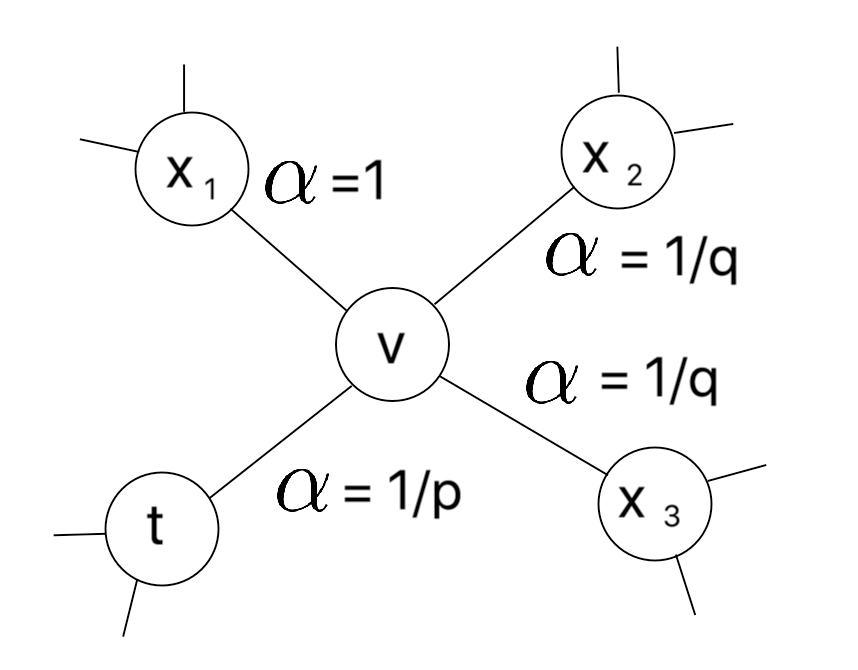
\includegraphics[width=0.5\linewidth]{plots/image2.png}
    \caption{Illustration   of   the   random   walk   procedure in node2vec. The walk from $t$ to $v$ is evaluating the next step.}
    \label{fig:my_label3}
\end{figure}

\section{Embedding Generation}
In case of text analysis study\cite{mikolov2013efficient} Skip-gram model is introduced for unsupervised representation learning of each word. Word2vec algorithm consist of the following steps. At first, set of word neighbors need to be collected. This can be easily achieved taking $context_size$ words before and $context_size$ words after considered word in the sentennce. After that, optimization problem maintaining neighbor words in a sentence close in an embedded feature space is formulated and solved using Stochastic Gradient Descent (SGD). That's how embedding representation of the words is obtained. 

node2vec utilizes \textbf{word2vec} algorithm. The idea behind utilization is \textbf{substitute neighbor words} in a text with \textbf{neighbor nodes} sampled during \textbf{random walk} process.

\section{Reference Implementation Caveats}
SNAP repository mentions two reference algorithm implementations written in Python and C++ respectively. Both two implementations store \textbf{precomputed transition probability matrix} in computer RAM and therefore show a good performance in cases of embedding small networks on a single machine. However that do not holds for large real-world networks containing tens of millions vertices. 

That problem can be tackled with running algorithm on a cluster of nodes. There is also a reference implementation utilizing Apache Spark distributed calculations framework. However \cite{zhou2018efficient} shows that it isn't also suitable for large networks. In addition, it has a limit of 30 edges for each node during the process of random walks generation that leads to generating poor embeddings.